\section{数据设计}
\label{sec:data_design}

\subsection{数据描述}
系统的数据设计需要同时服务三种目标：支持任务执行、支持结果回溯、支持系统治理。因此，数据不应只按“表存什么”理解，而应按“哪些对象支撑哪些设计行为”理解。结合前期需求分析，本系统的核心数据可以归纳为以下几类：
\begin{enumerate}[label=\arabic*.]
    \item 用户与权限数据：支撑角色识别、权限控制和菜单装载。
    \item 项目与场景数据：支撑项目管理、版本回溯和结果比较。
    \item 资产与资源数据：支撑生成、替换和风格联动。
    \item 布局与草图数据：支撑精确布局和草图驱动的空间调整。
    \item 任务与解析数据：支撑 LLM 理解、结构化任务生成和执行跟踪。
    \item 仿真与展示数据：支撑车辆、人群、船只等动态展示能力。
    \item 日志与审计数据：支撑故障定位、责任追踪和后台治理。
\end{enumerate}

从存储组织方式看，系统数据并不全部采用同一种结构保存。用户、角色、项目、任务状态和日志记录等信息适合采用结构化存储，以保证查询、过滤和审计效率；场景版本、布局结果、结构化任务内容和仿真配置等信息更适合采用半结构化存储，以保留复杂对象关系和可扩展字段；草图图像、场景文件和资源文件则以文件形式保存，并通过项目编号、场景版本编号或任务编号与结构化记录建立关联。这样的组织方式既能满足管理型数据的一致性要求，也能兼顾三维场景系统中复杂对象与外部文件共存的特点。

在数据转换路径上，系统首先将用户输入转化为可管理的数据对象，再根据对象类型进入不同处理链路。参数表单输入会直接形成结构化配置记录，草图和点线集会形成布局数据与中间识别结果，自然语言和多模态输入会形成解析记录与结构化任务，最终再与场景版本、仿真配置和日志记录建立关联。通过这一转换方式，系统能够将需求表达、任务执行和结果输出统一纳入可追踪的数据体系之中。

\subsection{数据流说明}
\begin{figure}[H]
\centering
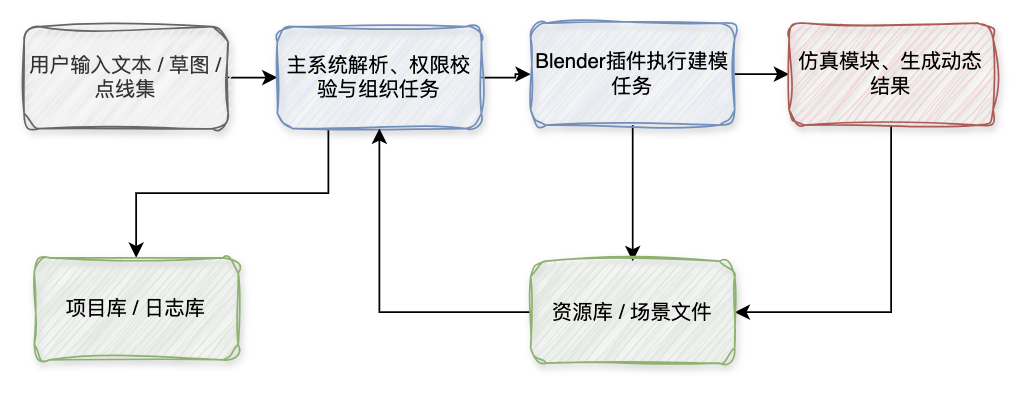
\includegraphics[width=\textwidth]{figures/8.png}
\caption{系统数据流图}
\label{fig:data_flow}
\end{figure}

从数据流角度看，用户输入先进入主系统进行规范化处理；之后输入被封装为任务并交给插件或 LLM 服务；执行结果回写场景和版本数据；仿真结果作为附加展示结果保存；关键过程同步写入日志。这样的设计可以将“输入、理解、执行、展示、审计”五个环节通过统一任务标识串联起来。

\subsection{核心实体设计}
\subsubsection*{1. 核心实体分组}
根据系统职责边界，核心实体可划分为五组。第一组为身份与权限实体，包括 \texttt{User}、\texttt{Role} 和权限相关记录，用于描述用户身份、访问边界和菜单装载规则；第二组为项目与场景实体，包括 \texttt{Project} 和 \texttt{SceneVersion}，用于描述项目生命周期以及多轮生成后的场景快照；第三组为资源与布局实体，包括 \texttt{Asset}、\texttt{LayoutSet} 和 \texttt{SketchImage}，用于表达生成所依赖的资源、空间控制信息和原始设计输入；第四组为任务与解析实体，包括 \texttt{Task} 和 \texttt{StructuredCommand}，用于连接用户意图、LLM 解析结果和插件执行过程；第五组为仿真与审计实体，包括 \texttt{SimulationPlan} 和 \texttt{OperationLog}，用于支撑动态展示与系统维护。

上述分组方式的目的，是将管理型对象、业务型对象和过程型对象区分开来。这样处理后，系统在实现时可以分别围绕用户治理、项目版本管理、场景执行链路和日志审计链路设计数据表、文件组织方式与接口输入输出格式，避免把所有数据混杂在同一层面中。

\subsubsection*{2. 核心实体与职责}
\begin{table}[H]
\centering
\caption{核心实体与职责}
\label{tab:core_entities}
\rowcolors{2}{gray!8}{white}
\begin{tabularx}{\textwidth}{p{2.2cm} p{1.8cm} p{2.2cm} Y}
\rowcolor{gray!20}
\toprule
实体 & 类型 & 主要存储形态 & 设计职责 \\
\midrule
User & 结构化实体 & 数据表/结构化记录 & 表示系统用户身份、账号状态与角色归属。 \\
Role & 结构化实体 & 数据表/结构化记录 & 表示角色类别及其对应权限集合。 \\
Project & 结构化实体 & 数据表/结构化记录 & 组织一个城市场景设计任务的生命周期。 \\
SceneVersion & 半结构化实体 & 结构化记录 + 场景文件关联 & 保存某次生成或修改后的场景状态快照。 \\
Asset & 半结构化实体 & 资源元数据 + 文件路径 & 记录资源类别、标签、路径、版本和适用条件。 \\
LayoutSet & 半结构化实体 & JSON/对象记录 & 描述点、线、面和控制参数构成的布局结果。 \\
SketchImage & 文件实体 & 图像文件 + 关联记录 & 保存用户上传草图及其识别关联信息。 \\
Task & 结构化实体 & 数据表/结构化记录 & 表示统一的可跟踪执行任务。 \\
StructuredCommand & 半结构化实体 & JSON/对象记录 & 表示解析后的对象、属性、关系与参数建议。 \\
SimulationPlan & 半结构化实体 & JSON/对象记录 & 保存动态对象配置与仿真参数。 \\
OperationLog & 结构化实体 & 日志表/结构化记录 & 保存关键操作、状态与异常信息。 \\
\bottomrule
\end{tabularx}
\end{table}

\subsubsection*{3. 实体关系说明}
核心实体之间存在较为明确的关联关系。一个 \texttt{User} 对应一个角色集合或角色标识，并以该角色参与项目创建、任务提交和后台管理等行为；一个 \texttt{Project} 可以关联多个 \texttt{SceneVersion}，用于记录同一项目在不同时间点的生成与修改结果；一个 \texttt{Task} 通常关联一次结构化任务内容、一次执行状态演化过程以及若干日志记录；一个 \texttt{SceneVersion} 可以引用多个 \texttt{Asset} 和一个或多个 \texttt{LayoutSet}，从而说明该版本场景由哪些资源和空间结构共同构成；当任务涉及动态展示时，还会进一步关联 \texttt{SimulationPlan}。

这种实体关系设计保证了系统能够回答几个关键问题：某个场景版本是由谁在什么项目中生成的、它依赖了哪些资源、它对应了哪次任务、任务经历了哪些状态变化、是否产生了动态仿真结果、出现异常时又应追溯到哪条日志记录。对软件设计而言，这些关系比单个字段本身更重要，因为它们决定了后续接口设计、数据库设计和对象建模时的主关联路径。

\subsection{数据字典}
{
\renewcommand{\arraystretch}{1.3}
\rowcolors{3}{gray!8}{white}
\begin{longtable}{p{2.5cm} p{1.8cm} p{2.0cm} p{6.0cm}}
\caption{主要数据字典}\label{tab:sdd_data_dict}\\
\toprule
\rowcolor{gray!20}
\textbf{数据项} & \textbf{类型} & \textbf{来源} & \textbf{说明} \\
\midrule
\endfirsthead
\toprule
\rowcolor{gray!20}
\textbf{数据项} & \textbf{类型} & \textbf{来源} & \textbf{说明} \\
\midrule
\endhead
\midrule
\multicolumn{4}{r}{\small 续下页}\\
\endfoot
\bottomrule
\endlastfoot
\texttt{user\_id} & 字符串 & 用户管理 & 用户唯一标识。 \\
\texttt{role\_type} & 枚举 & 权限模块 & 取值可为建模师、分析师、管理员。 \\
\texttt{project\_id} & 字符串 & 项目模块 & 项目唯一标识，用于组织场景与任务。 \\
\texttt{scene\_version\_id} & 字符串 & 场景模块 & 场景某次保存结果的唯一编号。 \\
\texttt{asset\_id} & 字符串 & 资产库 & 资产唯一标识，关联类别和资源路径。 \\
\texttt{layout\_payload} & JSON/对象 & 布局模块 & 保存道路、边界、区域等几何描述。 \\
\texttt{sketch\_path} & 文件路径 & 上传模块 & 草图文件位置，用于识别与追溯。 \\
\texttt{task\_id} & 字符串 & 调度模块 & 用于串联解析、执行、日志与结果。 \\
\texttt{task\_status} & 枚举 & 调度模块 & 典型状态包括待确认、排队中、执行中、成功、失败。 \\
\texttt{command\_spec} & JSON/对象 & LLM 模块 & 保存对象、属性、数量和空间关系等结构化结果。 \\
\texttt{sim\_config} & JSON/对象 & 仿真模块 & 保存动态对象数量、路径与速度等参数。 \\
\texttt{log\_message} & 文本 & 日志模块 & 保存关键操作或异常信息。 \\
\end{longtable}
}

\subsection{数据设计原则}
\begin{enumerate}[label=\arabic*.]
    \item 统一标识原则：项目、场景、任务和日志之间通过唯一编号建立关联。
    \item 版本保留原则：场景修改不直接覆盖，重要结果应沉淀为可回看版本。
    \item 过程可解释原则：LLM 解析结果要保留中间结构，而不仅是最终执行结果。
    \item 资源可管理原则：资产需要有类别、标签、版本和适用范围，便于筛选与治理。
\end{enumerate}
